\section{Results \& Discussion}\label{results}

% O =
%     4 0 4
% E =
%     739 131 50
%     589 690 92
%     302 571 664

In this section the obtained results are shown and discussed. Namely the results on the metrics the system measures.

\begin{figure}[ht]
    \centering
    \begin{subfigure}[t]{0.3\textwidth}
    \centering
    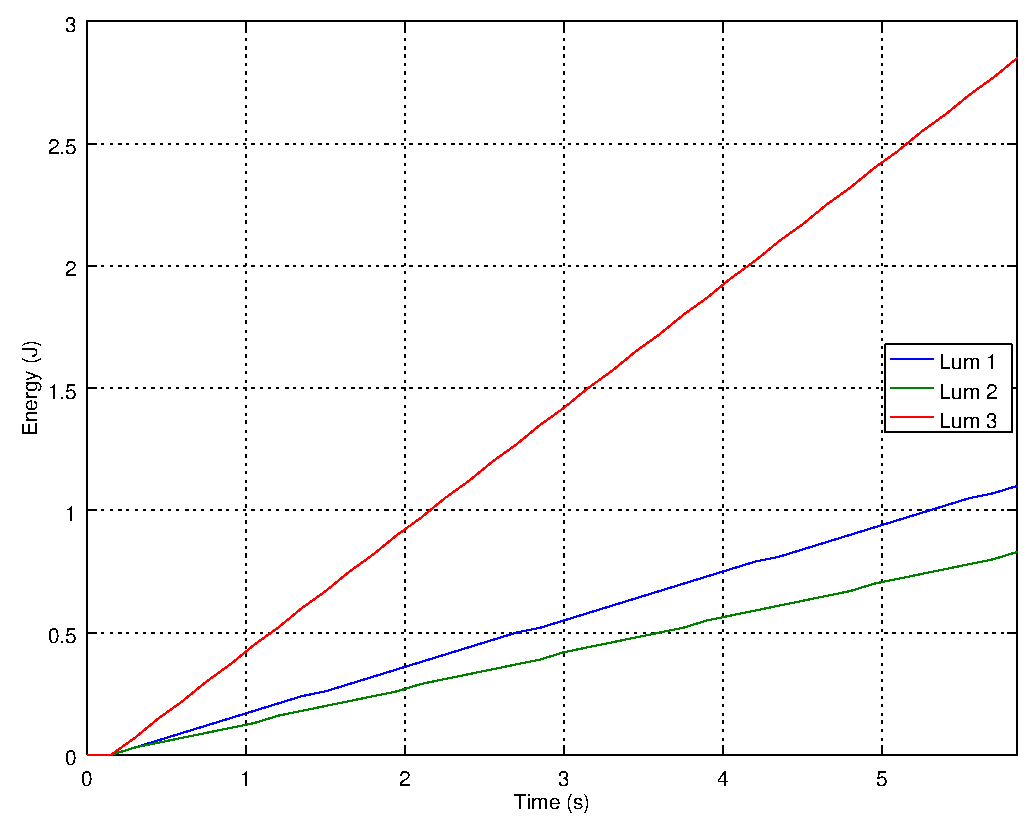
\includegraphics[width=.95\textwidth]{img/e_closed_o000}
    \caption{Energy over time of the 3 illuminaires.}
    \label{fig:e_closed_o000}
    \end{subfigure}
    \begin{subfigure}[t]{0.3\textwidth}
    \centering
    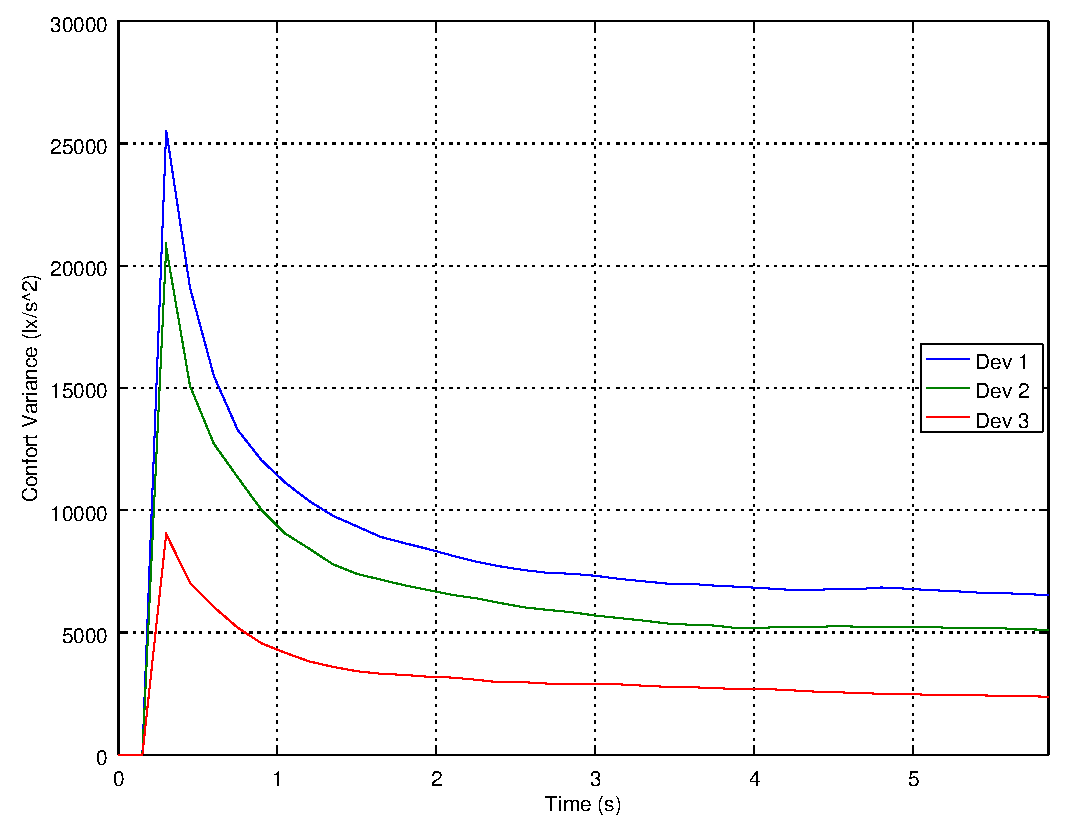
\includegraphics[width=.95\textwidth]{img/f_closed_o000}
    \caption{Confort variance over time of the 3 illuminaires.}
    \label{fig:f_closed_o000}
    \end{subfigure}
    \begin{subfigure}[t]{0.3\textwidth}
    \centering
    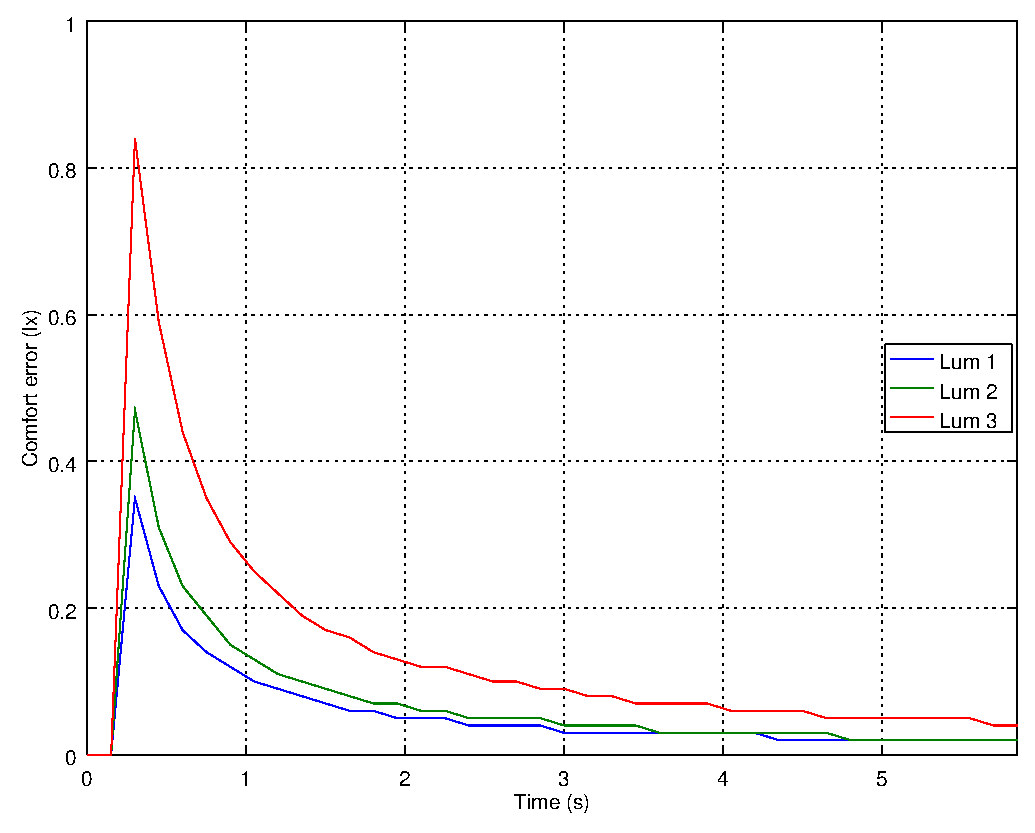
\includegraphics[width=.95\textwidth]{img/n_closed_o000}
    \caption{Confort error over time of the 3 illuminaires.}
    \label{fig:n_closed_o000}
    \end{subfigure}
    \caption{Metrics after system startup with the box closed and all desks as unoccupied. }
\end{figure}

%na justificação do conforto do 3 podes dizer que o steady state que mostra que conseguimos chegar até 50 luz foi tirado para o 1
%e o 3 para além de lhe faltar um bocado de papel por baixo é o unico que o LDR nao recebe luz directa do lado direito
%E dizer que a iluminação está lá (até está demais) o sensor é que não a apanha

\begin{figure}[ht]
    \centering
    \begin{subfigure}[t]{0.3\textwidth}
    \centering
    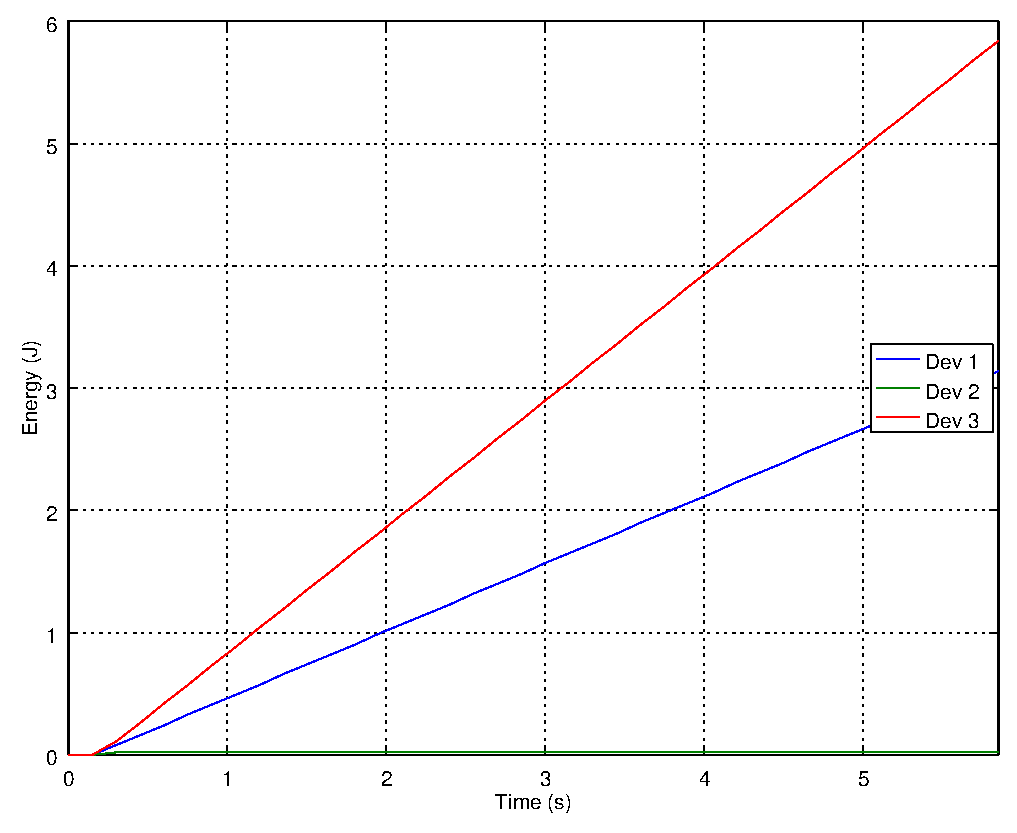
\includegraphics[width=.95\textwidth]{img/e_open_o101}
    \caption{Energy over time of the 3 illuminaires.}
    \label{fig:e_open_o101}
    \end{subfigure}
    \begin{subfigure}[t]{0.3\textwidth}
    \centering
    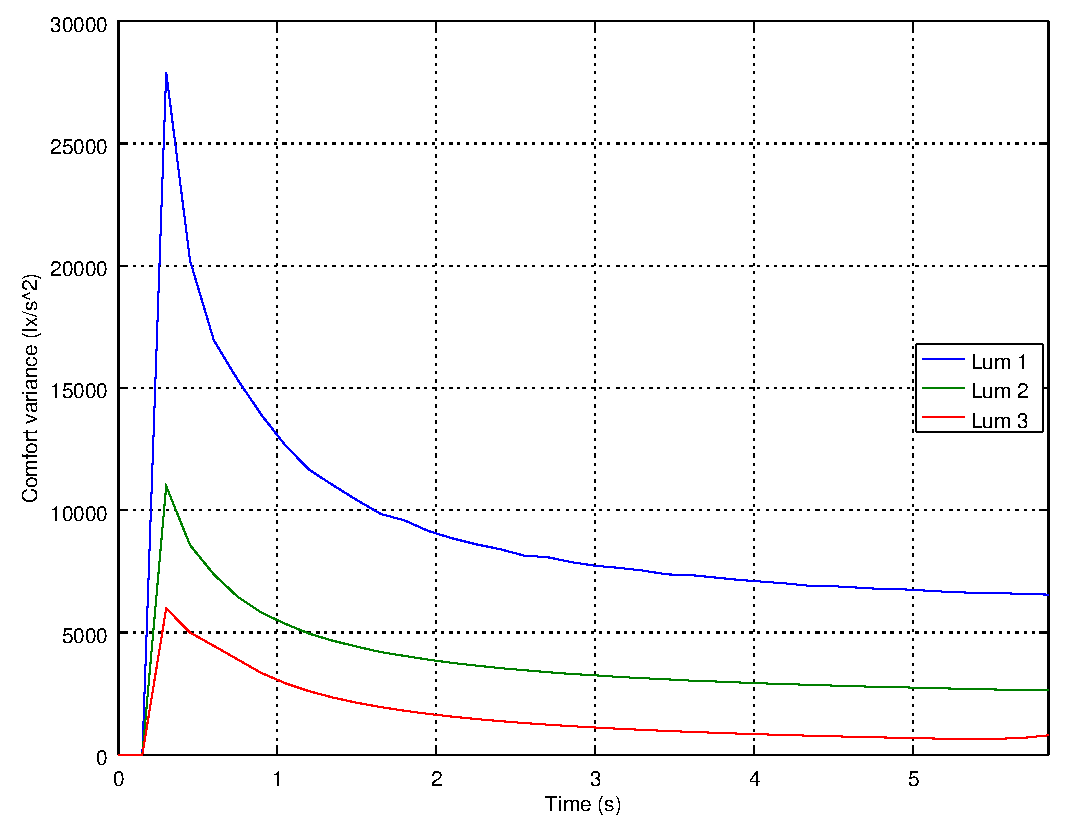
\includegraphics[width=.95\textwidth]{img/f_open_o101}
    \caption{Confort variance over time of the 3 illuminaires.}
    \label{fig:f_open_o101}
    \end{subfigure}
    \begin{subfigure}[t]{0.3\textwidth}
    \centering
    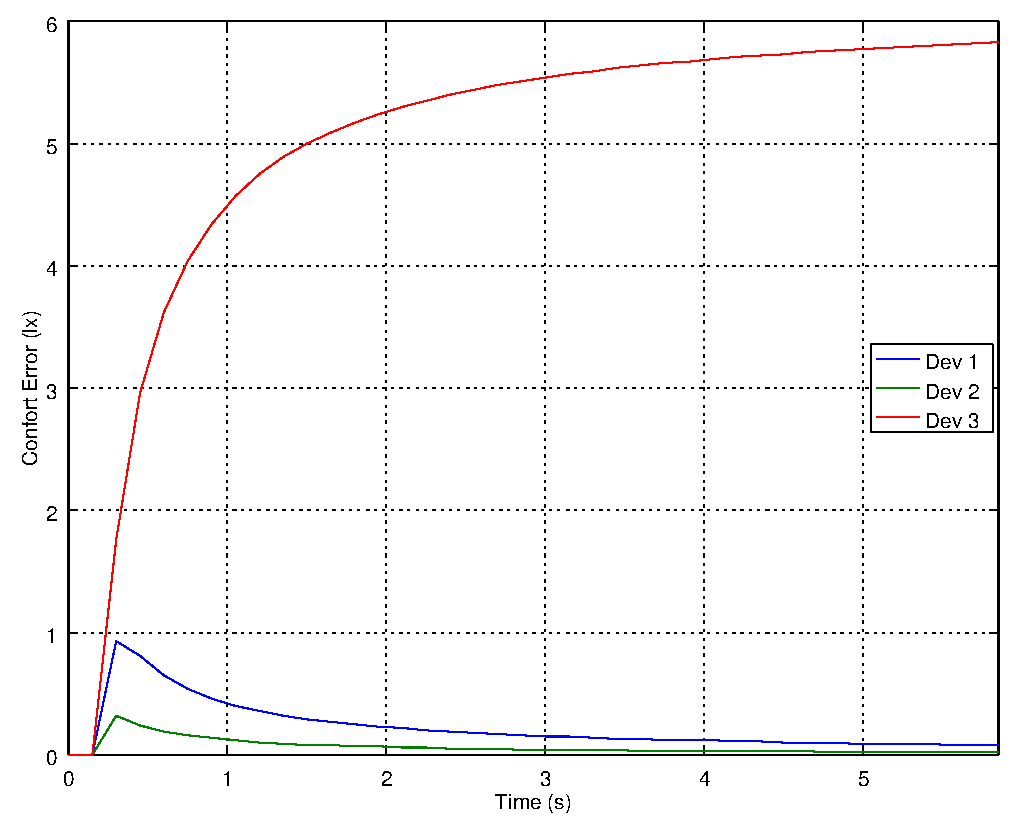
\includegraphics[width=.95\textwidth]{img/n_open_o101}
    \caption{Confort error over time of the 3 illuminaires.}
    \label{fig:n_open_o101}
    \end{subfigure}
    \caption{Metrics after system startup with the box open and desks 1 and 3 as occupied.}
\end{figure}


%\subsection{Energy}
%\subsection{Confort Error}
%\subsection{Confort Variance}
